\begin{tikzpicture}
\def\height{1} \def\pad{.3} \def\arrow{.7}\def\totalen{7}
\begin{scope}[xshift=-10cm, yshift=1.8cm,scale=.5]
    \fill [
        pattern={Lines[distance=2mm,angle=45,line width=0.7mm]},pattern color=black
       ] (0, \height) rectangle ++(\totalen, .5*\pad);
    \draw[top color = fluid, bottom color = white,draw=none] (0, 0) rectangle ++ (\totalen, -6*\pad);
    \draw[fill=pem, draw=none] (0, 0) rectangle ++ (\totalen, \height);

    \draw[black] (0, 0) -- ++ (\totalen, 0);
    \draw[black] (0, \height) -- ++ (\totalen, 0);
    \draw[<->] (-\pad, 0) -- ++ (0, \height) node[midway, left] {$h$};
    \draw[thick, <-] (\totalen/2, 0) -- ++ (210:4*\pad) node[left] {$p_i$};
    \draw[thick, ->] (\totalen/2, 0) -- ++ (-30:4*\pad) node[right] {$R$};
    \draw[dashed] (\totalen/2, 0) -- ++ (0, -4*\pad);
    \draw[<->] (\totalen/2, -2*\pad) arc (90:30:-2*\pad) node[midway, below] {$\theta$};
    
    \node at (-.7, 1.8){a)};
\end{scope}
\begin{scope}[xshift=-10cm, yshift=-1.5cm, scale=.5]
    \draw[top color = fluid, bottom color = white,draw=none] (0, 0) rectangle ++ (\totalen, -6*\pad);
    \draw[top color = white, bottom color = fluid,draw=none] (0, \height) rectangle ++ (\totalen, 6*\pad);
    \draw[fill=pem, draw=none] (0, 0) rectangle ++ (\totalen, \height);

    \draw[black] (0, 0) -- ++ (\totalen, 0);
    \draw[black] (0, \height) -- ++ (\totalen, 0);
    \draw[<->] (-\pad, 0) -- ++ (0, \height) node[midway, left] {$h$};
    \draw[thick, <-] (\totalen/2, 0) -- ++ (210:4*\pad) node[left] {$p_i$};
    \draw[thick, ->] (\totalen/2, 0) -- ++ (-30:4*\pad) node[right] {$R$};
    \draw[thick, ->] (\totalen/2, \height) -- ++ (30:4*\pad) node[right] {$T$};
    \draw[dashed] (\totalen/2, 0) -- ++ (0, -4*\pad);
    \draw[<->] (\totalen/2, -2*\pad) arc (90:30:-2*\pad) node[midway, below] {$\theta$};
    \node at (-.7, 3){b)};
\end{scope}

\begin{scope} 
    \node[draw=none,fill=none] at (0, 0){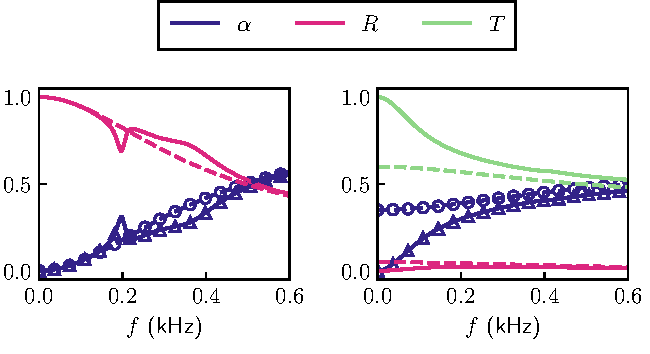
\includegraphics{poro_elastic_scattering.pdf}};
    \node at (-5.8, 1){c)};   
    \node at (-0.1, 1){d)};   
\end{scope}
\end{tikzpicture}